%
\documentclass{beamer}
\usepackage{caption}
\usepackage{subcaption}
\usepackage{arbenson-math}
\usepackage{graphics}
\usepackage{verbatim}

\graphicspath{{./figures/}}
\usetheme{boxes}
\usecolortheme{seahorse}

\AtBeginSection[]
{
  \begin{frame}<beamer>
    \frametitle{\thesection}
    \tableofcontents[currentsection]
  \end{frame}
}

\title{CME 193: Introduction to Scientific Python \\
Lecture 6: More on matrices}
\author{
Austin Benson \\
\vspace{0.1in}
Institute for Computational and Mathematical Engineering (ICME)}
\date{January 28, 2014}
\begin{document}

\maketitle

\section{Basic multiplication}

\begin{frame}
\frametitle{vector-vector dot product}

\[
\begin{pmatrix}
1 & 2 & 3 
\end{pmatrix}
\begin{pmatrix}
4 \\ 5 \\ 7
\end{pmatrix}
= 1 \cdot 4 + 2 \cdot 5 + 3 \cdot 7 = 35
\]

\codeblock{code/dot1.py}

\end{frame}

\begin{frame}
\frametitle{Matrix-vector multiplication}

\[
\begin{pmatrix}
1 & 2 & 3  \\
3 & 2 & 1
\end{pmatrix}
\begin{pmatrix}
4 \\ 5 \\ 7
\end{pmatrix}
= \begin{pmatrix}
1 \cdot 4 + 2 \cdot 5 + 3 \cdot 7 \\
3 \cdot 4 + 2 \cdot 5 + 1 \cdot 7 \\
\end{pmatrix}
= \begin{pmatrix}
35 \\
29 \\
\end{pmatrix}
\]

\codeblock{code/dot2.py}

\end{frame}

\begin{frame}
\frametitle{Matrix-matrix multiplication}

\[
\begin{pmatrix}
1 & 2 & 3  \\
3 & 2 & 1
\end{pmatrix}
\begin{pmatrix}
4 & 1 \\ 5 & 1 \\ 7 & 0 \\
\end{pmatrix}
= \begin{pmatrix}
35 & 3 \\ 29 & 5 \\
\end{pmatrix}
\]

\[
\begin{pmatrix}
1 & 2 & 3  \\
3 & 2 & 1
\end{pmatrix}
\begin{pmatrix}
4 \\ 5 \\ 7
\end{pmatrix}
= \begin{pmatrix}
35 \\
29 \\
\end{pmatrix} \text{ (last slide)}
\]

\[
\begin{pmatrix}
1 & 2 & 3  \\
3 & 2 & 1
\end{pmatrix}
\begin{pmatrix}
1 \\ 1 \\ 0
\end{pmatrix}
= \begin{pmatrix}
1 \cdot 1 + 2 \cdot 1 + 3 \cdot 0 \\
3 \cdot 1 + 2 \cdot 1 + 1 \cdot 0 \\
\end{pmatrix}
= \begin{pmatrix}
3 \\
5 \\
\end{pmatrix}
\]

\codeblock{code/dot3.py}

\end{frame}

\begin{frame}
\frametitle{Stacking}

\begin{itemize}
\item \texttt{vstack}: "vertical stack"
\item \texttt{np.vstack((A, B))} $\to \begin{pmatrix} A \\ B \end{pmatrix}$
\end{itemize}
\begin{itemize}
\item \texttt{hstack}: "horizontal stack"
\item \texttt{np.hstack((C, D))} $\to \begin{pmatrix} C & D \end{pmatrix}$
\end{itemize}

\end{frame}

\begin{frame}
\frametitle{Stacking}

\codeblock{code/stack1.py}

\end{frame}

\begin{frame}
\frametitle{Stacking}

Careful!!

\texttt{
Traceback (most recent call last): \\
  File "stack1.py", line 10, in <module> \\
    print np.dot(A, B) \\
ValueError: objects are not aligned
}

\codeblock{code/stack2.py}

$B = \begin{pmatrix} 4 & 5 & 7 & 1 & 1 & 0 \end{pmatrix}$

\end{frame}

\begin{frame}
\frametitle{Stacking: transpose problems}

\codeblock{code/stack4.py}

\end{frame}

\begin{frame}
\frametitle{Vectors}

The transpose of numpy vectors are vectors! (1-dimensional)

\codeblock{code/stack5.py}

\end{frame}

\begin{frame}
\frametitle{Vectors $\to$ matrices}

Need to convert to matrices

\codeblock{code/stack6.py}

\end{frame}

\begin{frame}
\frametitle{Working transposes}

\codeblock{code/stack7.py}

\end{frame}

\begin{frame}
\frametitle{Other subtleties}

\codeblock{code/subtle1.py}

\pause

\begin{center}
[6 6] [6 6]

[4 8] [4 8]
\end{center}

\end{frame}


\begin{frame}
\frametitle{Other subtleties}

\codeblock{code/subtle2.py}

\pause

\begin{center}
[[0 0]

 [0 0]]
\end{center}

\end{frame}


\begin{frame}
\frametitle{Other subtleties}

\codeblock{code/subtle3.py}

\pause

\begin{center}
[[ 0.5  0.5]

 [ 0.5  0.5]]
\end{center}

\end{frame}


\section{QR}

\begin{frame}
\frametitle{$n \times n$ QR}

\begin{itemize}
\item $A$ is $n \times n$
\item $A = QR$, $Q$, $R$ $n \times n$
\item $Q^TQ = I$
\item $R_{ij} = 0$ if $i > j$: "upper triangular"
\end{itemize}

\begin{figure}
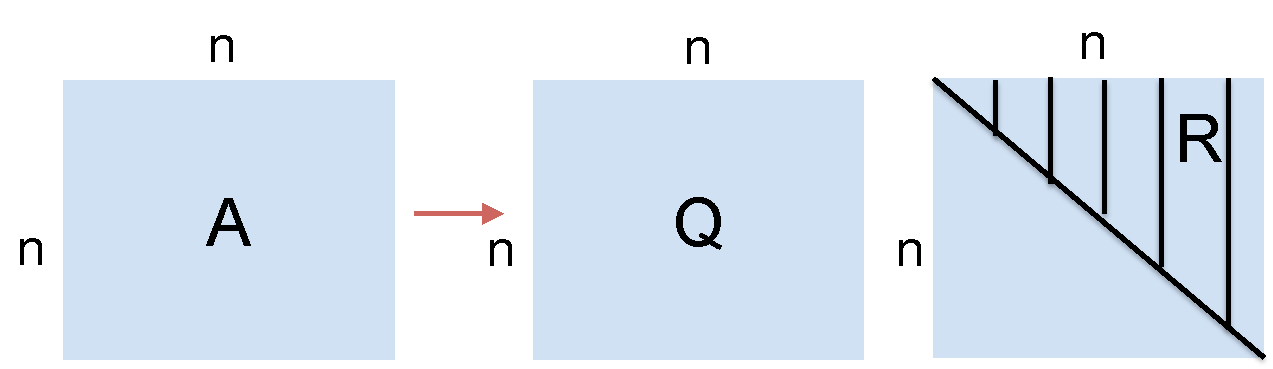
\includegraphics[scale=0.4]{figs/qr.pdf}
\end{figure}

\end{frame}


\begin{frame}
\frametitle{$m \times n$ QR}

\begin{itemize}
\item $A$ is $m \times n$, $m > n$
\item $A = QR$, $Q$ $m \times n$, $R$ $n \times n$
\item $Q^TQ = I$
\item $R_{ij} = 0$ if $i > j$: "upper triangular"
\end{itemize}

\begin{figure}
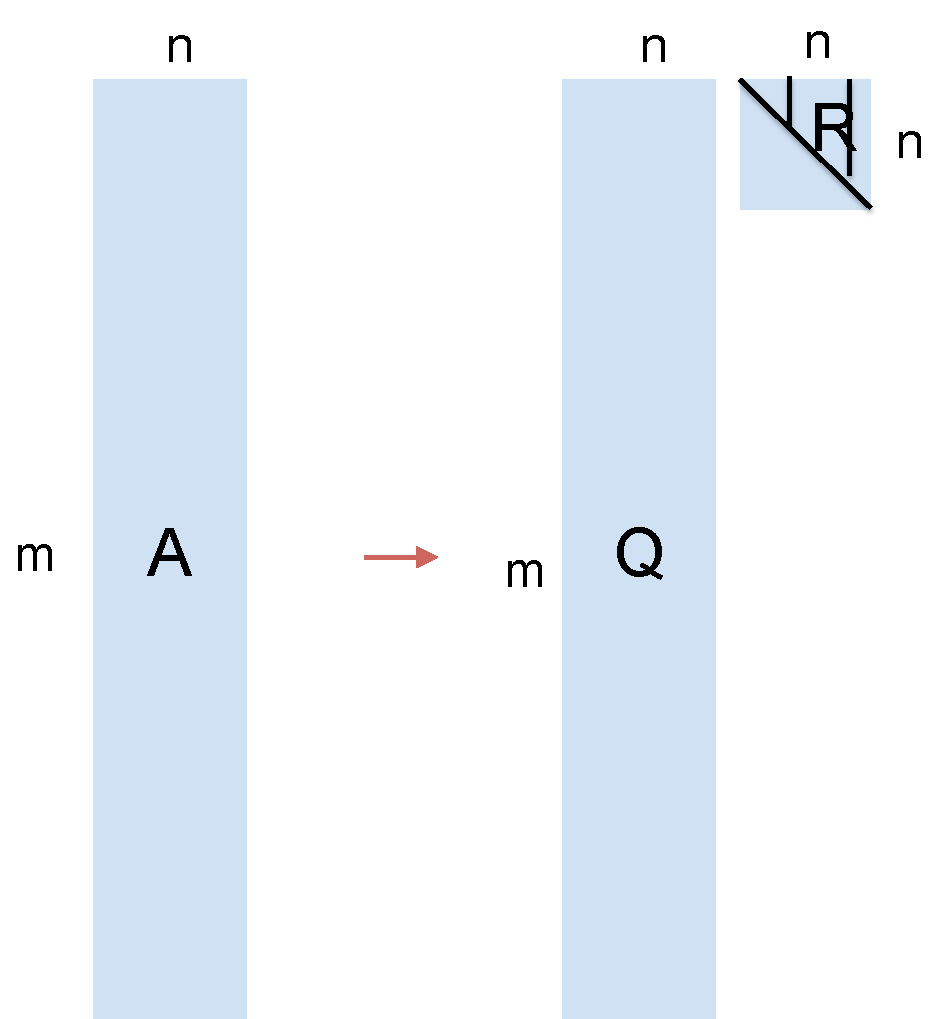
\includegraphics[scale=0.3]{figs/tsqr.pdf}
\end{figure}

\end{frame}

\begin{frame}
\frametitle{Least squares}

\begin{itemize}
\item Have several input vectors $x_1$, $x_2$, $\ldots$, $x_n$, each of length $m$.
\item Have a one output vector $y$ of length $m$
\item Want find vector $\beta$ to minimize
\[
 \ssum{i=1}{m} \ssum{j=1}{n}(x_{ij}\beta_j - y_j)^2
 \]
\end{itemize}

\begin{figure}
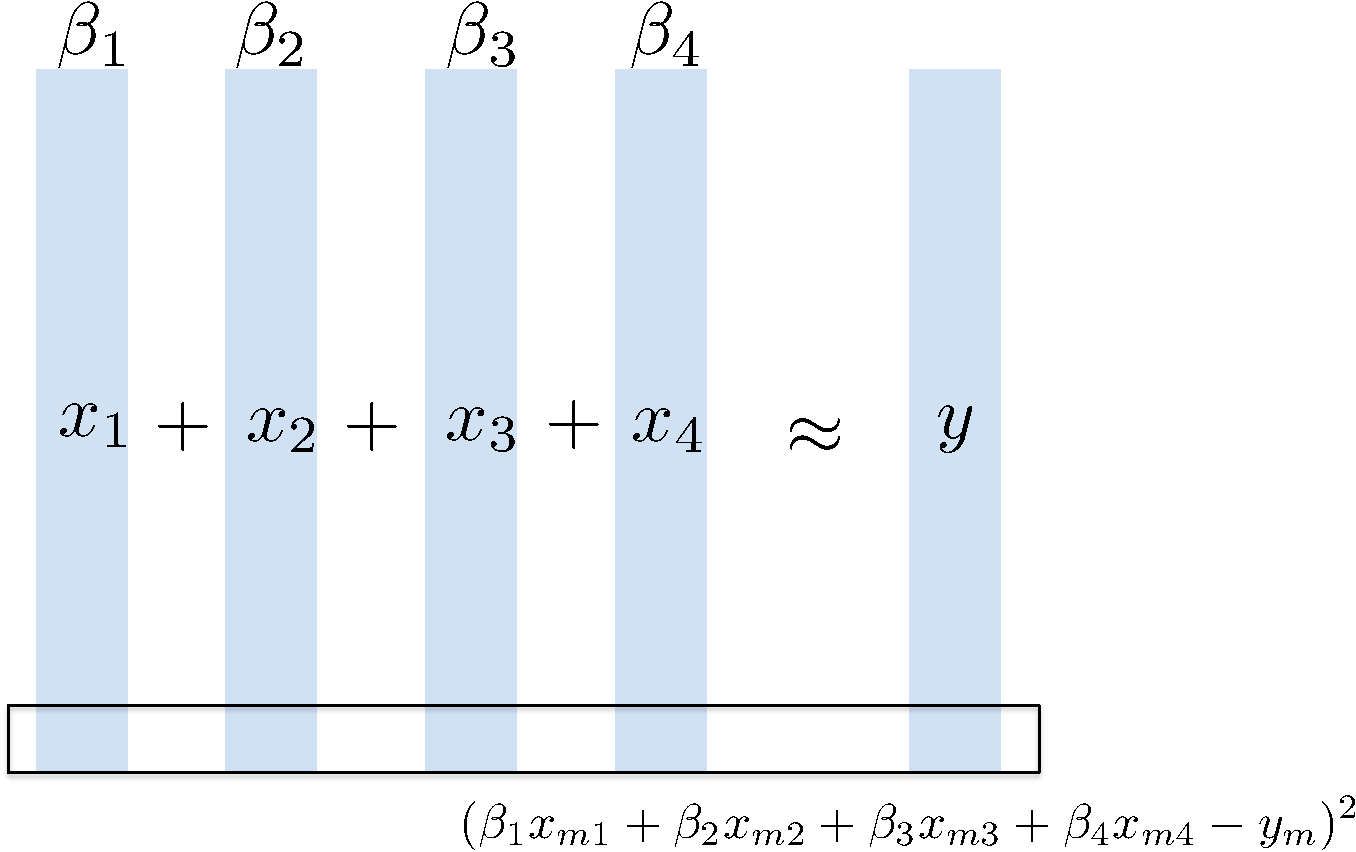
\includegraphics[scale=0.3]{figs/lstsq.pdf}
\end{figure}

\end{frame}

\begin{frame}
\frametitle{Matrix form of least squares}

Matrix form:

\[
\min_{\beta} (X\beta - y)^T(X\beta - y)
\]

\vspace{1cm}

\begin{itemize}
\setlength{\itemsep}{0.5cm}
\item $X = \begin{pmatrix} x_{11} & \hdots & x_{1n} \\ & \vdots \\ x_{m1} & \hdots & x_{1n}\end{pmatrix} = \begin{pmatrix} x_1 \\ \vdots \\ x_m \end{pmatrix}$
\item $\beta = \begin{pmatrix}\beta_1 \\ \vdots \\ \beta_n\end{pmatrix}$,
$y = \begin{pmatrix}y_1 \\ \vdots \\ y_m\end{pmatrix}$
\end{itemize}

\end{frame}

\begin{frame}
\frametitle{Least squares}

\[
\hat{\beta} = \min_{\beta} (X\beta - y)^T(X\beta - y)
\]

\begin{itemize}
\item $X = QR$
\item $z = Q^Ty$
\item $R\hat{\beta} = z$
\end{itemize}

\vspace{1cm}

Moral of the story: QR has a purpose

\end{frame}

\begin{frame}
\frametitle{NumPy least squares}

\begin{enumerate}
\item $X = QR$
\item $z = Q^Ty$
\item $R\hat{\beta} = z$
\end{enumerate}

\codeblock{code/qr1.py}

\end{frame}


\begin{frame}
\frametitle{NumPy + SciPy QR}

\begin{enumerate}
\item $X = QR$
\item $z = Q^Ty$
\item $R\hat{\beta} = z$
\end{enumerate}

\codeblock{code/qr2.py}

\end{frame}


\begin{frame}
\frametitle{NumPy least squares}

\codeblock{code/qr3.py}

\end{frame}

\section{SVD}

\begin{frame}
\frametitle{SVD}

The singular value decomposition (SVD) of a matrix $A$:
\begin{itemize}
\item $A$ is $n \times n$
\item $A = U\Sigma V^T$, all $n \times n$
\item $U^TU = V^TV = I$
\item $\Sigma$ is diagonal with $\Sigma_{ii} \ge \Sigma_{jj} \ge 0$ for $i < j$.
\end{itemize}

\begin{figure}
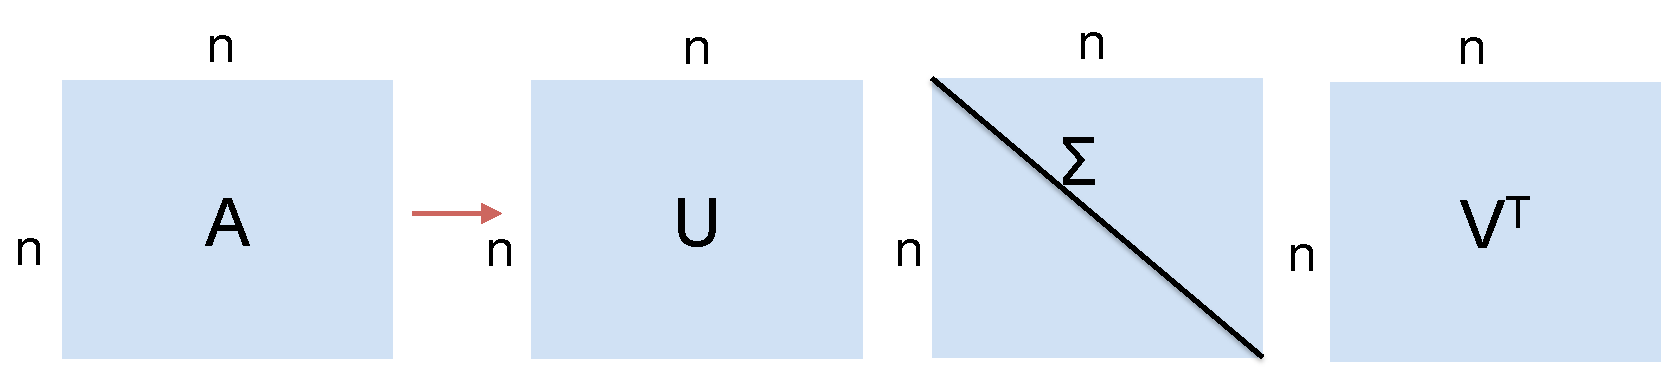
\includegraphics[scale=0.4]{figs/svd.pdf}
\end{figure}

\end{frame}

\begin{frame}
\frametitle{SVD: applications}

SVD appears all over the place, for example:

\vspace{1cm}

\begin{itemize}
\item Principal component analysis
\item Low-rank approximations in computational physics
\item Signals processing
\end{itemize}

\end{frame}


\begin{frame}
\frametitle{SVD example}

\codeblock{code/svd1.py}

\begin{figure}
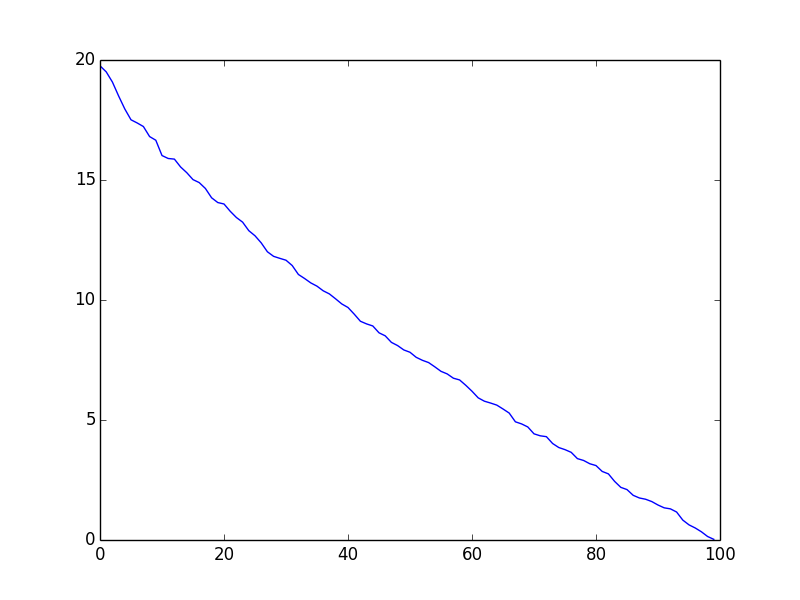
\includegraphics[scale=0.25]{figs/svd_plot.png}
\end{figure}

\end{frame}

\begin{frame}
\frametitle{SVD example}

\codeblock{code/svd2.py}

\begin{figure}
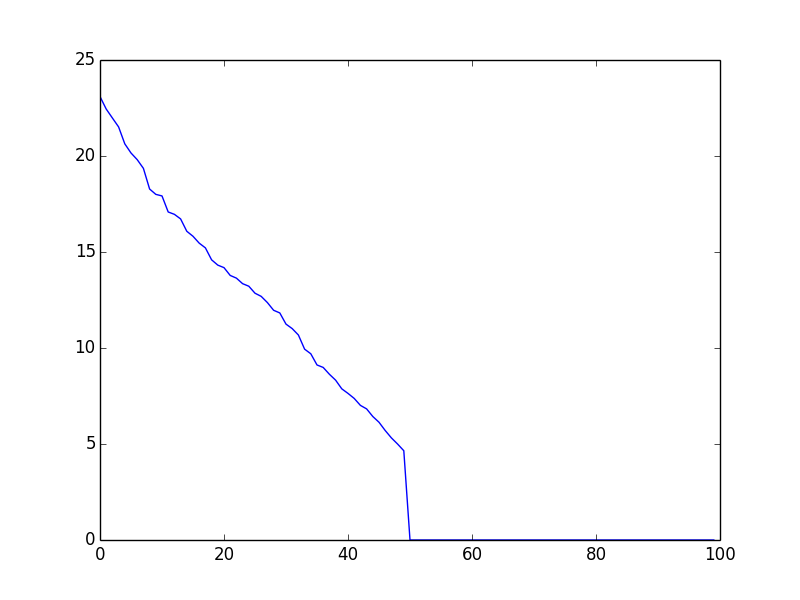
\includegraphics[scale=0.2]{figs/svd_lowrank.png}
\end{figure}


\end{frame}


\end{document}
